\chapter{Environnement}

Dans ce chapitre, nous allons présenter l'environnement dans lequel nous avons
développé les deux projets. Il va aussi servir à introduire un ensemble de
règles et de conventions utilisées par la suite.
Nous présenterons également les technologies utilisées au cours de ce projet.

    \section{Réunions et contacts}

Tout au long du projet, nous avons été en contact permanent avec Mr Berry,
que ce soit par e-mails, appels téléphoniques ou réunions. Ces dernières
étaient quasi-hebdomadaires, afin de rester le plus possible dans la
bonne direction. Nos recontres ont eu lieu à Polytech' ou au Lirmm.

    \section{Gestionnaire de versions}

Dès le balbutiement du projet, nous avons décidé d'utiliser un gestionnaire
de version. En effet, celui-ci nous permettait d'avoir un contrôle total des modifications
tout au long du développement.

Notre choix s'est naturellement porté sur Git \cite{git}. Cela s'explique 
par les aspects suivants:

    \begin{itemize}
    \item Multi-plateformes.
    \item Gestions des branches.
    \item Développement actif et forte communauté d'utilisation.
    \item Rapidité d'éxécution comparé à svn, hg, etc. 
    \end{itemize}

    De plus certains d'entre nous l'avait déjà utilisé précédement: git est assez
    complèxe à prendre en main au début cependant l'entraide était de mise.

    Mais surtoût, le plus important pour nousreste quand même le site web GitHub \cite{github}.
    Il fait office de serveur centralisé pour git. Mais pas seulement puisqu'il 
    propose entre autre:

    \begin{itemize}
    \item L'hébergement de projets sous Git
    \item Des fonctionnalités de type réseaux sociaux, dont :
        \begin{itemize}
        \item Les flux
        \item Le suivi de personnes ou de projets
        \item Les graphes de réseau pour les dépôts
        \end{itemize}
    \item Un pastebin nommé Gist
    \item Un wiki et une page web pour chaque dépôt
    \end{itemize}

C'est un site web qualifié de professionnel puisqu'il est utilisé par de 
nombreux projets de grandes tailles tels que : Git, Perl, Facebook, Twitter,
JQuery, PHP, Python, etc.

De plus, Mr Berry, de part le Lirmm, ne pouvait nous ouvrir qu'un serveur
Subversion, donc Git couplé avec GitHub est un excellent compromis.

Nota Bene : son adoption sous les systèmes Windows relève encore du portage
expérimental. Il a été codé par le créateur de Linux, pour versionner le code
de ce dernier, et s'utilise par conséquent en lignes de commandes.

    \section{Règles de codage}

Ci-dessous, voici les règles de codage utilisées tout au long du projet
ainsi que dans le rapport. Elles sont là pour permettre une cohérence tout au
long du développement, mais aussi et surtout, pour que la relecture et la 
compréhension soient simplifiées pour les développeurs du projet, ainsi que pour les
futures personnes amenées à travailler dessus.

Cela regroupe:

    \begin{itemize}
    \item Un code en anglais (commentaire compris).
    \item Eviter de dépasser 80 caractères si possibles.
    \item Indentation de 4 espaces, pas de tabulation.
    \end{itemize}

Ci-dessous, un fichier C++ d'exemple.

\begin{lstlisting}
#ifndef BADGER_FOO_HPP
#define BADGER_FOO_HPP

#include <string>

namespace badger
{
///////////////////////////////////
/// \brief Sample class
///
/// Use for example.
///////////////////////////////////
class FooBar
{
public:
virtual const int& doSomething() const = 0;

private:
int m_attribute;
};

} // namespace badger

#endif //BADGER_FOO_HPP
\end{lstlisting}

    \section{Technologies utilisées}

        \subsection{C++}

    // Victor

        \subsection{CMake}

CMake \cite{cmake}, pour "Cross platform Make", est un programme qui permet à partir 
de scripts uniques, de générer l'ensemble des fichiers de constructions standard 
du programmes, et celà, comme son nom l'indique, de manière multi-plateformes.

En effet, CMake est capable de créer projets pour Visual Studio ou XCode, et même 
des Makefiles; et cela pour bon nombre de compilateurs (msvc, gcc, clang, etc) et 
de plateformes (Windows, MacOS, Linux, BSD, etc). Cela est possible grâce au
système de générateur de CMake.

    \begin{figure}[h]
        \begin{center}
        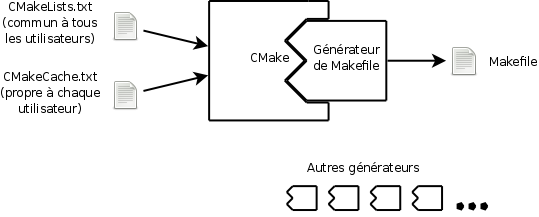
\includegraphics[scale=0.4]{images/CMakeFonctionnement.png} 
        \end{center}
        \caption{Fonctionnement de CMake}
        \label{Fonctionnement de CMake}
     \end{figure} 

Il est comparable au programme SCons ou aux Autotools.

C'est un projet en développement constant, puisque la dernière version date du 19
avril 2012. De plus de nombreux projets reconnus l'utilisent, comme Bullet, Ogre
ou encore KDE.

Les scripts décrivant les projets sont écris dans les fichiers CMakeLists.txt.
Ci-dessous, un exemple minimal pour compiler un projet.

    \lstset{language=Bash}
    \begin{lstlisting} 
cmake_minimum_required(VERSION 2.6)
		
# Configuration
project(my_project)
set(EXECUTABLE_OUTPUT_PATH bin/${CMAKE_BUILD_TYPE})

file(GLOB_RECURSE source_files src/*)

add_executable(my_exe ${source_files})
    \end{lstlisting}

Le programme CMake s'utilise soit en lignes de commandes, soit avec une un logiciel
possèdant une IHM.

Dans le projet, nous avons utilisés ce système de génération pour le programme 
gérant la communication avec le lecteur de carte.

        \subsection{xHTML / CSS}

Le xHTML (extensive HyperText Markup Langage) et le CSS (Cascade Style Sheet) sont
des langages de description, et non des langages de programmation.
Ces deux langages sont complémentaires, le HTML sert à représenter ``le fond'', le contenu
en lui même, alors que le CSS représente ``la forme'', c'est le design du site, permettant
une mise en page entièrement configurable via le système de balises du code HTML.

Il s'agit de deux langages simples à apprendre, car il s'agit uniquement d'imbriquer des
balises pour le HTML, et d'affecter des propriétés de styles à ces balises dans le CSS.
Toutefois, la réalisation d'un design agréable et fonctionnel n'est pas une tâche aisée,
aussi, nous avons reçu de l'aide pour le style graphique.

        \subsection{PHP}

PHP \cite{php} (PHP: Hypertext Preprocessor) est un langage de programmation interprété que l'on écrit
dans des fichiers de script à l'extension .php. Ce langage est interprété par le serveur
et permet principalement la génération de pages web dynamiques.

Nous avons principalement utilisé le fait que PHP est devenu un langage objet dans sa dernière version
ce qui nous a permis de construire une architecture basée sur l'héritage pour notre framework.
En plus de la programmation orientée objet, nous avons utilisés de nombreuses fonctionnalités avancées
de la librairie standard.

        \subsection{Javascript / AJAX}

// William

        \subsection{SQL / MySQL}

// William

        \subsection{Java}

// Jamal
